\documentclass[a4paper,11pt,report]{scrartcl}
\usepackage[dutch]{babel}
\usepackage[T1]{fontenc}
\usepackage[utf8]{inputenc}
\usepackage{lmodern}
\usepackage{amssymb}
\usepackage{color}
\usepackage{graphicx}
\usepackage{mathtools}
\DeclareGraphicsExtensions{.pdf,.png,.jpg}
\newcommand{\tab}{\hspace*{2em}}

\title{\huge\textbf{Deliverable 4}}
\subtitle{\textbf{TI2206 Software Engineering Methods\\
Delft University of Technology\\
The Netherlands}}
\author{Piet van Agtmaal 4321278\\
	    Jochem Heijltjes 1534041\\
		Arthur Hovanesyan 4322711\\
		Paul Bakker 4326091\\
		Jente Hidskes 4335732
	   }


\begin{document}
\begin{titlepage}
\maketitle
\thispagestyle{empty} %geen page numbering op opening pagina
\end{titlepage}

\newpage\section{Preamble}

The document you are currently reading is the report for deliverable four of group 21.\\

Group 21 consists of the members 
Piet van Agtmaal, Jochem Heijltjes, Arthur Hovanesyan, Paul Bakker and Jente Hidskes.\\
We are five Computer Science students at the Delft University of Technology,
The Netherlands. We created a clone of the original 2048 game for the course
Software Engineering Methods.\\

The goal of this course is to teach us how to develop software by applying the most appropriate software engineering practices, given the context of development.\\
We were asked to make a clone of the game 2048, then apply several design strategies to it and add a few extra features. This report covers what we have done, why and how.\\

We would like to thank our teacher Dr. Bachelli and our Teaching Assistants Moritz Beller and Aimee Ferouge for guiding us through this project.\\

Thank you for taking interest in this report. We hope you will enjoy reading our report and playing 2048!

\newpage\section{Introduction}

2048 is a very popular game created by by Gabriele Cirulli, based on 1024 by
Veewo Studio and conceptually similar to Threes by Asher Vollmer.\\
For this project we were asked to create a clone of the game 2048 in the Object-Oriented programming language Java, so that's what we did!\\

We didn't just make a clone of the original 2048 game, we also added
multiplayer functionality, automatic solvers allowing you to play against the computer and 
undo/redo functionality. 
Now you can challenge your computer, your neighbours, your
coworkers, your kids or even the Queen of England to play a game of 2048!\\

The purpose of this report is to present how we implemented several features/techniques and why they were implemented.\\
This document tells you everything you need to know about our project and to get you started playing 2048. Technical aspects of the game are covered in here as well.\\

 The structure of this report is as follows. Chapter three describes how to play 2048 and all the functionalities that are implemented. The next chapter explains how the the application is tested and how quality is being ensured. Chapter six covers the design patterns we have implemented including the corresponding class and sequence diagrams. The next chapter, chapter 7 will explain the extra design pattern we have chosen, why and how we implemented it.\\
Finally, chapter eight will conclude this report. \\

\newpage\section{How to play 2048}

This section briefly describes how to play 2048 and provides information on
the functionality it has, such as playing the game alone, with friends and how
to use the logging features.

\subsection{Singleplayer game}
After starting the application you will see the main menu. In the main menu,
click the \texttt{Singleplayer} button to start your singleplayer game.\\

Using the arrow keys you can move the tiles on the grid. Each time two tiles with the same
number collide, the numbers are added and the two tiles merge. Your goal is to
reach the 2048 tile!\\

To return to the menu, press \texttt{Escape} any time. Don't worry,
your current game will be saved for you! (This also applies to closing the
game!).

\subsection{Multiplayer game}
The multiplayer version is identical to the singleplayer, except here you will
compete against a friend, colleague, coworker or your worst enemy over LAN or
the internet. Your opponent does not have to be in the same room with you; they
can even be on the other side of the planet and you can still kick their
asses!\\

Your goal is to reach the 2048 tile and get more points than your opponent.  In case you
are unable to reach the 2048 tile (e.g., because you lost), your opponent will either win or lose if they have more points. 

In case your grid is full, you will need to wait for your opponent to make the last move on their grid.

We will now briefly explain how to connect to eachother. Please refer to the
documentation of your networking equipment or software in case you experience
networking problems.

\subsubsection{Joining a game}
To connect to another player, choose the \texttt{Join a game} option in the
main menu. The application will try to connect to the remote address you
entered, on port 2048, using TCP.

\subsubsection{Hosting a game}
To have another player connect to you, choose the \texttt{Host a game} option
in the main menu. The application will bind to port 2048/TCP on all the
system's network interfaces. In case you wish to play over the internet,
please make sure connections on this port are forwarded to your local address
on your NAT device. Consult the manual of your network products for more 
information.


\subsection{Challenging your computer}

You can now challenge and play against your computer. After starting the game, you will see the main menu. In the main menu, pick the option \texttt{Challenge me!}. In the next menu you can select the difficulty you want to play on.\\

Depending on your selection, the computer will make moves at a timed interval. The higher the difficulty you select, the shorter the computer will wait between moves and the better calculated its movements are.\\

The solver algorithm behind the \texttt{Easy} option is able to win about 15\%, but only one move is made every after 1.6 second. The same algorithm is used for the other options, but it will be more accurate when trying to make a new move. The solver will solve at least 35\% of the grids with 650 milliseconds between each move with the \texttt{Extreme} option.

If either player (you or the computer) ends up with a full grid, the game will wait for the other to complete the game before finally announcing either of you winner or loser.\\

Whoever has the highest amount of points in the end wins the game.

\subsection{Logging}
The game supports several commandline arguments for logging.\\

By default, the application will log to the standard output, using the
\texttt{ALL} logging level. If enabled, however, errors will be logged to
\texttt{stderr}. The logging level can also be adjusted.\\

The supported arguments are:
\begin{verbatim}
$ jarfile.jar [logLevel] [file]
\end{verbatim}
or, otherwise:
\begin{verbatim}
$ Launcher.java [logLevel] [file]
\end{verbatim}
Both of these fields are parsed case-insensitively.\\

Two examples:
\begin{verbatim}
$ Launcher.java debug
\end{verbatim}
will run the game and log all debug and info messages. 
\begin{verbatim}
$ Launcher.java error file
\end{verbatim}
will run the game and log all debug, error and info messages to the system's
output streams (\texttt{stdout} and \texttt{stderr}) and will write them to a
new file as well.\\

Please see the corresponding section below for more information on the possible
arguments:\\

\textbf{logLevel} can be one of the following:
\begin{description}
	\item[all] logs all messages;
	\item[info] logs info messages only;
	\item[error] log error messages and info messages;
	\item[debug] log debug, error and info messages;
	\item[none] disables logging.
\end{description}

\textbf{file}

Setting the \texttt{file} flag will write all messages of the previously set
logging level to a file. By default, a new file with the format
\texttt{2048\_YYYYMMDD\_HHmmss.log} will be created, where
\texttt{YYYMMMDDD\_HHmmss} is the time of application start.

\newpage\section{Test report}

In this section we will explain how we tested our game. We will start by
explaining how often we tested our game. Afterwards, we will explain what
kinds of testing we have done. Lastly, we will present the results of the
testing procedure.

\subsection{Test frequency}
In this section we will discuss how frequently we tested our game. Due to the
design patters we implemented, testing was essential. We tested using our
unit tests (locally and on Devhub as well) and visual tests. Implementing
iterators caused some problems that only arised during our visual tests. These
were, however, resolved immediately.

\subsection{Testing methods}
Visual tests involved actually playing the game and analyzing logging output
manually. Unit tests simply check object properties with certain input.

\subsection{Test results}
EclEmma is the tool we used for analyzing and measuring our test coverage.
As before, we analyzed our entire project using three different metrics: line,
branch and instruction coverage.\\

The results are as follows:
\begin{description}
	\item Line coverage: 73.0\%
	\item Branch coverage: 66.9\%
	\item Instruction coverage: 71.3\%
\end{description}
As with previous deliverables, we faced the same issues with code that requires
graphically rendering our game. 

\subsection{Conclusion}
Although our test results are lower than we had planned to achieve, we believe
our project has again been tested sufficiently.

\newpage\section{Exercise 1 - 20-Time}
In this section we will describe what we have implemented as extra feature.

We implemented the following extra features:
\begin{description}
	\item Automatic grid solving and playing against the computer
	\item Undo and redo functionality
\end{description}

We choose to implement an automatic grid solving feature because the idea seemed challenging to us. Two members of team tried to implement their own algorithm. Both are included in the production code, however, because one of them isn't entirely finished it's only implemented for hinting the player into a direction in Single player mode.\\
The other solver is capable of solving at least 35\% of the grids. However, only the "Challenge me!" mode, where the player will compete against the computer, fully utilizes this solver algorithm.\\

The undo and redo functionality is part of the Single player mode to give the player the opportunity to correct mistakes when trying to solve the puzzle. We chose to implement this feature because one of our team members likes this feature on the original game and he's unable to solve any puzzle without it. :P

\newpage\section{Exercise 2 - Design patterns}
In this section we will discuss the two chosen design patterns. Per pattern,
we will provide (in natural language) a description of why and how the pattern
is implemented, together with a class- and sequence diagram.

\subsection{The Command pattern}
We implemented the command pattern because we wanted to undo and redo the movements made by the player. After deciding to implement the command pattern we also wanted to make commands for the movements, as every move was a clear command.

\subsubsection{The implementation}
We have decided to make the \texttt{Command} class an abstract class as there where pieces of code that was used in every command so it would be beneficial to have that code in the Command class as a method.  The invoker of a command is the \texttt{InputHandler} class. It will invoke the command using the standard method: 
\begin{verbatim}
execute()
\end{verbatim}
We have made a command for every direction of movement for the grid. These command have as a receiver the \texttt{TileHandler} class. \texttt{TileHandler} preforms the actual actions of moving the tiles in the grid.\\

We have also made a command for undo and a command for redo. These commands have as a receiver the class \texttt{Grid}. The \texttt{Grid} class keeps two stacks of strings, one stack keeps track of the previous grid when a move is made and the other stack keeps track of the grid before an undo command is executed. The undo and redo command pop a string of the correct stack and sets it as the current grid. This is all done in the method:
\begin{verbatim}
execute()
\end{verbatim}


\newpage
\subsubsection{The class- and sequence diagram}
\textbf{The class diagram:}\\
\centerline{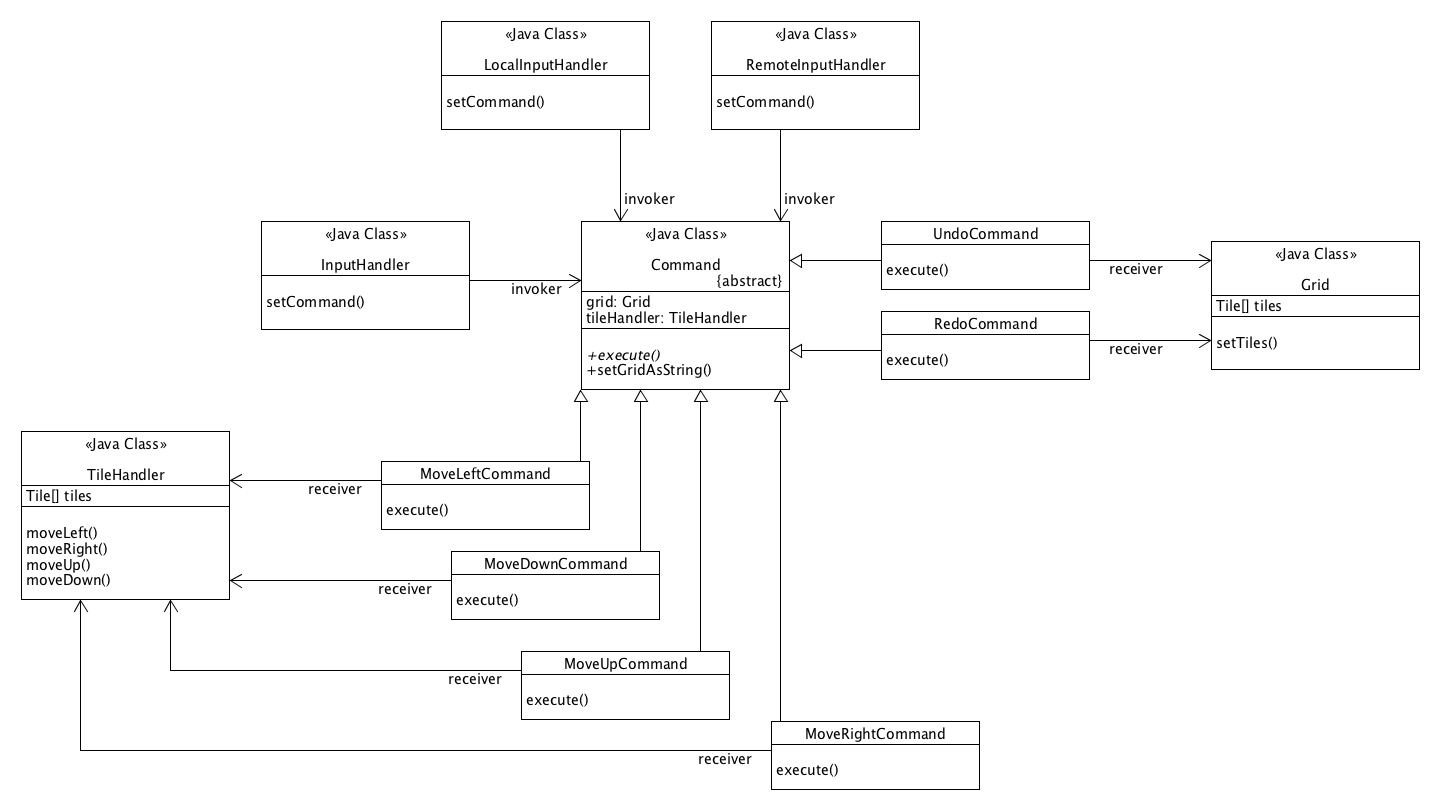
\includegraphics[scale=0.4]{commandPatternUML}}

\newpage\textbf{The sequence diagram:}\\
\centerline{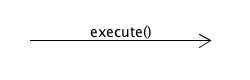
\includegraphics[scale=0.5]{commandPatternSequence}}

\newpage\subsection{The State pattern}
Blablabla

\subsubsection{The implementation}

\newpage\subsubsection{The class- and sequence diagram}
\textbf{The class diagram:}\\
\centerline{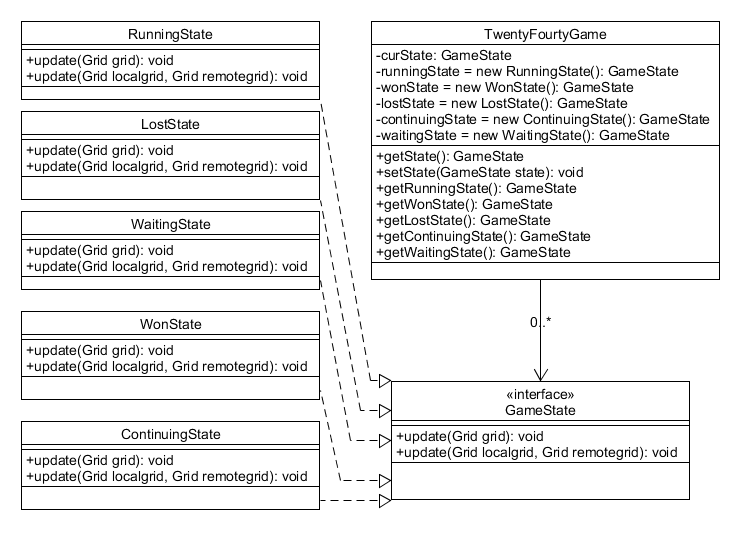
\includegraphics[scale=0.7]{statePatternUML}}

\newpage\textbf{The sequence diagram:}\\
\centerline{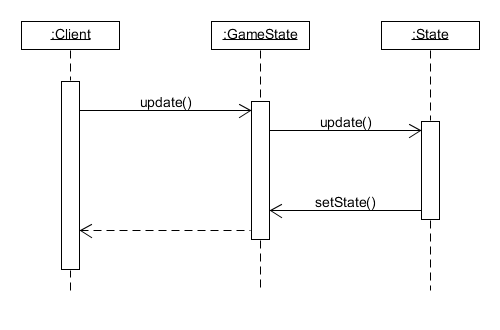
\includegraphics[scale=1]{statePatternSequence}}

\newpage\section{Exercise 3 - One more design pattern}
\subsection{The MVC pattern}
\subsubsection{The implementation}

\newpage\subsubsection{The class- and sequence diagram}
\textbf{The class diagram:}\\
\centerline{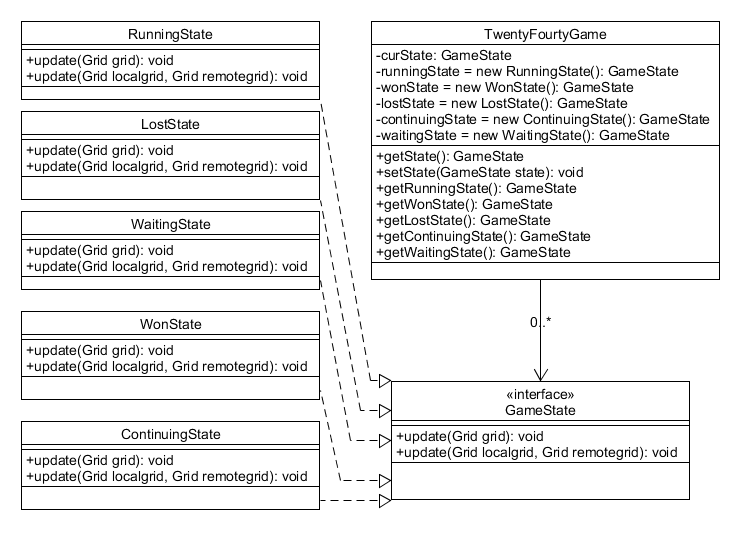
\includegraphics[scale=0.7]{statePatternUML}}

\newpage\textbf{The sequence diagram:}\\
\centerline{\includegraphics[scale=0.7]{MVCsequence2}}


\centerline{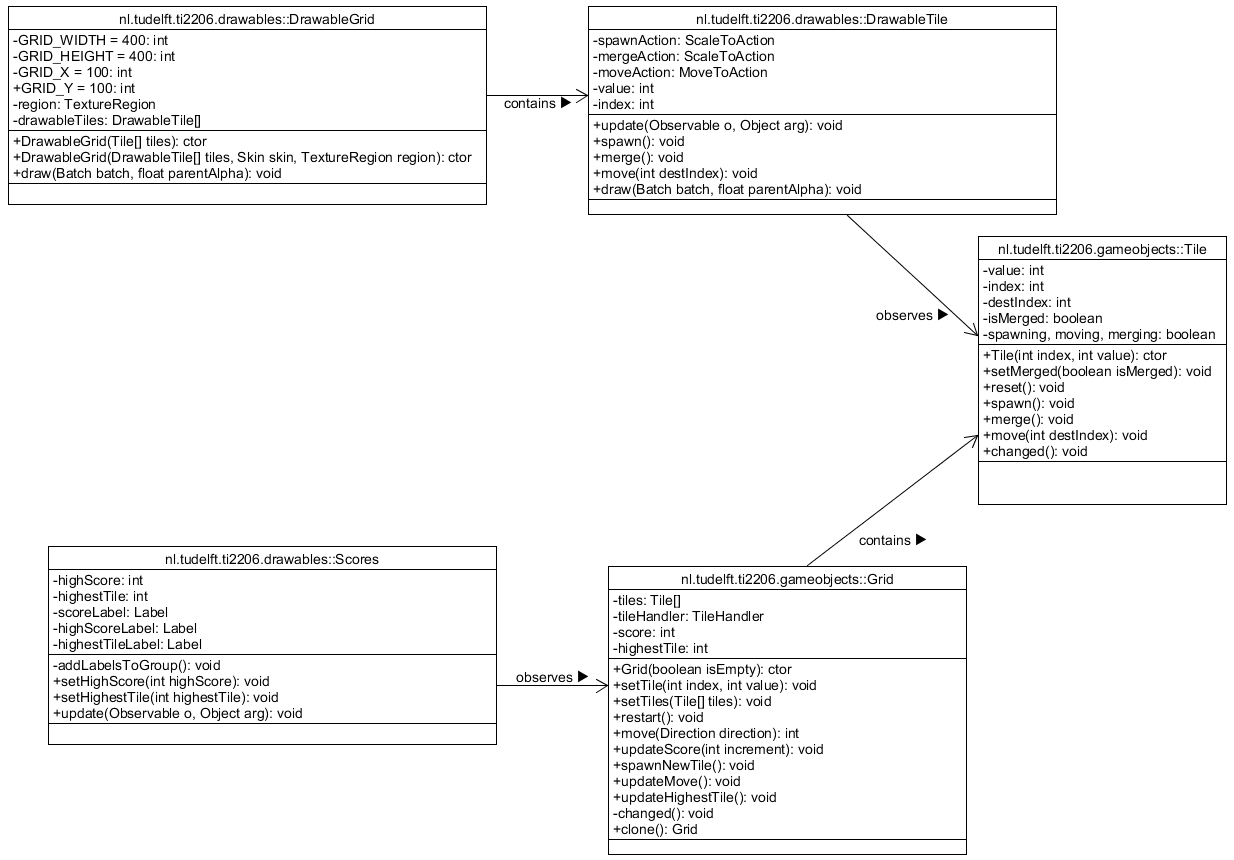
\includegraphics[scale=0.7]{mvcPattern}}

\newpage\section{Conclusion}

The goal of this report was to explain how we developed our 2048 clone, how and why we implemented several features. 
The development of the game was shown to have been undertaken in several consecutive steps. First of all we created just a fully working clone of the original 2048 game. Then, we implemented a multiplayer mode where the player can play against others over the network. After that we refactored our entire game and implemented several design patterns and added several extra features we thought of ourselves.

The three extra features we implemented were:
- Automatic grid solving 
- Playing against the computer 
- Undo and redo functionality

The latest design pattern we implemented is the MVC (Model-View-Controller) pattern.

We hope you enjoyed reading this report. Have fun playing 2048!

\end{document}
